\documentclass[letterpaper,twocolumn,amsmath,amsfont,amssymb,english,aps,jcp,preprintnumbers,groupaddress,nofootinbib,tightenlines]{revtex4}

\usepackage{graphicx}
\usepackage{epstopdf}

%\documentclass[aps,prb,letterpaper,twocolumn,nofootinbib,showkeys]{revtex4-1}
%\documentclass[aps,amssymb,prl,letterpaper,twocolumn,nofootinbib,showkeys]{revtex4-1}

%\usepackage[backend=bibtex]{biblatex}

%    backend=biber,
%    style=authoryear,
%    natbib=true,
%    sortlocale=en_US,
%    url=false,
%    doi=true,f
%    eprint=false
%]{biblatex}
%\usepackage{hyperref}


\newcommand{\mat}[1]{\boldsymbol{#1}}
\newcommand{\mmat}[1]{\widetilde{\boldsymbol{#1}}}
\newcommand{\matT}[1]{\boldsymbol{#1}^\dagger}
\newcommand{\ot}{ {\scriptstyle \otimes}_{ \tau } }

%\hypersetup{pdftitle={FreeON Project Report 1}}
%\hypersetup{pdfauthor={Matt Challacombe and Nicolas Bock}}
%\hypersetup{pdfsubject={A SpAMM Stabilized Newton Schulz Preconditioner: Fighting Error with Error}}

%\bibstyle{aipnum4-1}

\begin{document}

\title{On Stability of Newton Schulz Iterations in an Approximate Algebra}

\author{Matt Challacombe}
\email{matt.challacombe@freeon.org}
\homepage{http://www.freeon.org}
\affiliation{Theoretical Division, Los Alamos National Laboratory}

\author{Nicolas Bock}
\email{nicolasbock@freeon.org}
\homepage{http://www.freeon.org}
\affiliation{Theoretical Division, Los Alamos National Laboratory}

%\begin{abstract}
%Forward look
%\end{abstract}

\maketitle
\section{Introduction}

In many areas of application, finite correlations lead to matrices with decay properties.  By decay, we mean an approximate 
(perhaps bounded \cite{}) inverse relationship between matrix elements and an associated distance;  this may be a simple inverse 
exponential relationship between elements and the Cartesian distance between support functions, or it may 
involve a generalized distance, {\em e.g.}~ a statistical measure between strings.  
In electronic structure,  correlations manifest in decay properties of the gap shifted matrix 
sign function, as projector of the effective Hamiltonian (Fig.~\ref{figure1}).  
More broadly, matrix decay properties may coorespond to statistical matrices 
\cite{penrose1974,voit00,Anselin2003,Hardin2013,Krishtal2014}, including learned correlations in a 
generalized, non-orthogonal metric \cite{}. More broadly still, problems with local, non-orothogonal support 
are often solved with congruential transformations of the matrix inverse square root \cite{Lowdin56,naidu11} or a related factorization \cite{Krishtal2014};
these transformations correlate local support with a representation independent form, {\em eg.}~of the eigenproblem. 
Interestingly, the matrix sign function and the matrix inverse square root function are related by Higham's identity:
\begin{equation}
\rm{sign} \left( \begin{bmatrix} 0 & \mat{s}      \\ \mat{I}       & 0\end{bmatrix} \right)  =
                 \begin{bmatrix} 0 & \mat{s}^{1/2} \\ \mat{s}^{-1/2} & 0\end{bmatrix}  .
\end{equation}
A complete overivew of matrix function theory and computation is given in Higham's enjoyable reference \cite{Higham08}. 

A well conditioned matrix $\mat{s}$ may often correspond to matrix sign and inverse square root functions with rapid exponential decay, 
and be amenable to the sparse matrix approximation
$\bar{\mat{s}} = \mat{s}+ \mat{\epsilon}^{\mat{s}}_\tau$, where $\mat{\epsilon}^{\mat{s}}_\tau$ is the error introduced according to some  
criteria $\tau$.  Supporting this approximation are usefull bounds to matrix function elements \cite{Benzi99b, }.  
The criteria $\tau$ might be a drop-tolerence, 
$\epsilon^{\mat{s}}_{\tau} = \{-s_{ij}*\hat{\mat{e}}_i \, | \, |s_{ij}|<\tau \}$, a radial cutoff, 
$\epsilon^{\mat{s}}_{\tau} = \{-s_{ij}*\hat{\mat{e}}_i \, | \, \lVert \mat{r}_i - \mat{r}_j \rVert > \tau \}$, 
or some other approach to truncation, perhaps involving a sparsity pattern chosen {\em a priori}. 
Then, conventional computational kernels may be employed, such as the sparse general matrix-matrix multiply 
($\tt{SpGEMM}$) \cite{Gustavson78, Toledo97,challacombe00,bowler00}, yeiding fast solutions for multiplication rich iterations and a modulated fill in. 
These and related incomplete/inexact approaches to the computation of sparse approximate matrix functions often lead to ${\cal O}(n)$ 
algorithms, finding wide use in technologically important preconditioning schemes, the information sciences, electronic structure and many
other disciplines.  Comprehensive surveys of these methods in the numerical linear algebra are given by Benzi \cite{Benzi99,Benzi02}, and
by Bowler \cite{Bowler12} and Benzi \cite{Benzi13} for electronic structure.

\begin{figure}[t]\label{figure1}
 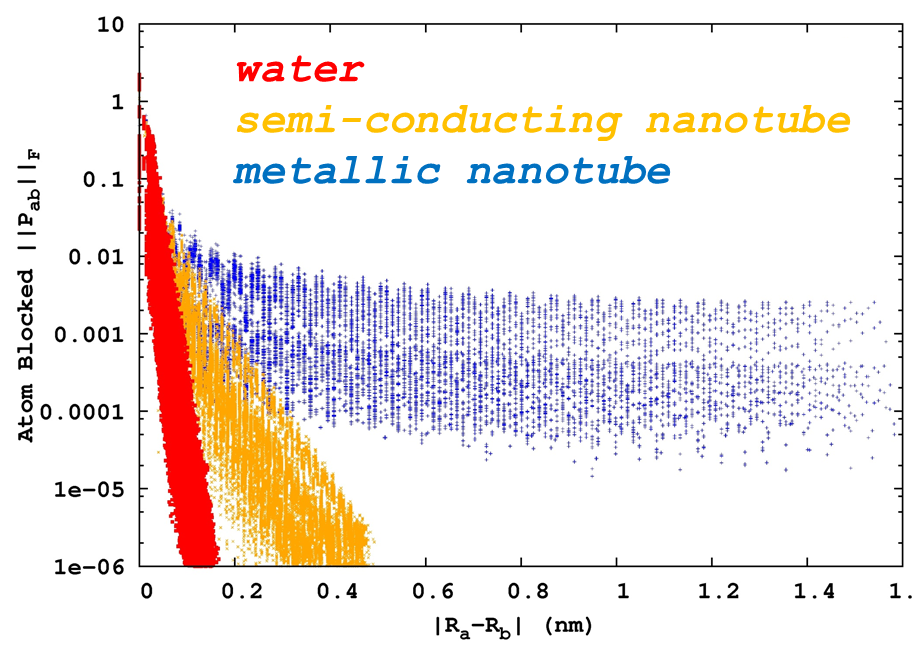
\includegraphics[width=3.5in]{decay_picture.png}
  \caption{Examples from electronic structure of decay for the spectral projector (gap shifted sign function) with respect to local (atomic) support.  
           Shown is decay for systems with correlations that are short (insulating water), medium (semi-conducting 4,3 nanotube), and 
           long (metalic 3,3 nanotube) ranged,  from exponential (insulating) to algebraic (metallic). }
\end{figure}

Because the truncated multiplication is controled only by absolute, addititve errors in the  product,   
\begin{equation} \label{sparseapprox}
\overline{ \mat{a} \cdot \mat{b} }\; = \; \mat{a}\cdot\mat{b} \; +\; \mat{\epsilon}^{\mat{a}}_\tau \cdot \mat{b} \;+\;
 \mat{a} \cdot \mat{\epsilon}^{\mat{b}}_\tau  \; + \;   {\mathcal O}(\tau^2)
\end{equation}
achieving sparse, stable and rapidly convergent iteration for ill-conditioned problems can be challenging \cite{}.  In cases of 
extreme degeneracy,  hierarchical semi-seperable (reduced rank) algorithms  can offer effective complexity reduction \cite{}.
However, many pratical cases are somewhere in-between sparse and meaningfully degenerate regimes; effectively dense but without
an exploitable reduction in rank.  This is the case in electronic structure for strong but non-metalic correlation, 
{\em e.g.}~towards the Mott transition \cite{}, and also in the case of local atomic support towards completeness \cite{Others, Hutter, Gigi}. 

\pagebreak
In this contribution, we consider an $N$-body approach to the approximation of matrix functions with decay, 
based on the quadtree data structure \cite{wise, samet} 
\begin{equation}
\mat{a}^i = \begin{bmatrix} \,  \mat{a}^{i+1}_{00} \, & \,  \mat{a}^{i+1}_{01} \,  \\[0.2cm]  \, \mat{a}^{i+1}_{10} \,  & \,\mat{a}^{i+1}_{11} \, \end{bmatrix} \, ,
\end{equation}
and orderings that are locality preserving \cite{}.  Orderings that preserve data locality are well developed in the
database theory \cite{}, providing fast spatial and metric querries.  
Locality enabled, fast data access is central to the $N$-Body approximation \cite{}, and an important problem 
for enterprise \cite{} and runtime systems \cite{}, with memory hierarchies becoming increasingly assynchronous and decentralized \cite{cache}.  
For matrices with decay, orderings that preserve locality lead to block-by-magnitude matrix structures with well 
segregated neighborhoods, inhabited by matrix elements of like size, and efficiently resolved by the quadtree data structure \cite{}.

With block-by-magnitude ordering of matrices $\mat{a}$ and $\mat{b}$, 
the Sparse Approximate Matrix Multiplication ($\tt SpAMM$) kernel,  $\ot$, carries out fast 
occlusion culling of insignifcant volumes in the product octree:
\begin{widetext}
\begin{equation}
\mat{a}^{i} \ot \mat{b}^{i} = 
\left\{
        \begin{array}{ll}
                 \emptyset \quad \tt{if}\quad \lVert \mat{a}^i \rVert \lVert \mat{b}^i \rVert < \tau \\[0.2cm]
                 \mat{a} ^i \cdot \mat{b}^i \quad  \tt{if}(i=\tt{leaf}) \\[0.2cm]
\begin{bmatrix} \mat{a}^{i+1}_{00} \ot \mat{b}^{i+1}_{00} +\mat{a}^{i+1}_{01} \ot \mat{b}^{i+1}_{10} \; , \; &
                \mat{a}^{i+1}_{00} \ot \mat{b}^{i+1}_{01} +\mat{a}^{i+1}_{01} \ot \mat{b}^{i+1}_{11}  \\[0.2cm] 
                \mat{a}^{i+1}_{00} \ot \mat{b}^{i+1}_{01} +\mat{a}^{i+1}_{01} \ot \mat{b}^{i+1}_{11} \; , \; & 
                \mat{a}^{i+1}_{00} \ot \mat{b}^{i+1}_{01} +\mat{a}^{i+1}_{01} \ot \mat{b}^{i+1}_{11}   
\end{bmatrix}  \quad \tt{else}
                \end{array}
              \right.  \, ,
\end{equation}
\end{widetext}
with errors linear in $\tau$ 
bounded by the sub-multiplicative norms $\lVert \cdot \rVert \equiv \lVert \cdot \rVert_F$ and the Cauchy-Schwarz inequality \cite{kahan,}.
In Ref.\cite{Challacombe2014}, we generalize this recursive task occlusion to the problem of Fock exchange.

The approximate $\tt SpAMM$ product is 
\begin{equation}
\widetilde{\mat{a}\cdot \mat{b}} \,  \equiv \, \mat{a} \ot \mat{b} \, 
  = \, \mat{a} \cdot \mat{b} + \mat{\Delta}^{a \cdot b}_{\tau} 
+ {\cal{O}} \left(  \tau^2 \right) \; ,
\end{equation}
with the culled contractions $\mat{\Delta}^{a \cdot b}_{\tau}$ obeying the $\tt SpAMM$ bound 
\begin{equation}\label{bound}
\lVert \mat{\Delta}^{a \cdot b}_{\tau} \rVert \, \leq \, \tau \, \lVert \mat{a} \rVert  \,  \lVert \mat{b} \rVert \, , 
\end{equation}
at each level of recursion.  This makes $\ot$ {\em stable}, as defined by Demmel, Dumitriu and Holz (see Eq.(1), Ref.~\cite{Demmel07}). 
However, instead of the roundoff error, we are concerned with the deterministic $\tt SpAMM$ error,  which 
leads to a non-associative algebra and error flows with properties of the Lie bracket
\begin{equation}
\widetilde{\left[ \mat{a} , \mat{b} \right]} \equiv \mat{a} \ot \mat{b}-\mat{b} \ot \mat{a}  
=  \left[ \mat{a} , \mat{b} \right]
+ \mat{\Delta}^{a\cdot b}_{\tau} -\mat{\Delta}^{b\cdot a}_{\tau} \,.
\end{equation}
The interesting group theory associated with the construction of matrix functions is developed by Higham, Mackey, Mackey and T 
in Ref.\cite{}.  
%In this contibution, we consider only the magnitude of these error flows.     

$\tt SpAMM$ is similar to compressed kernels for sketching the matrix product \cite{Kutzkov2012, Pagh2013}. 
spatial join! Paugh.  MAD.  etc    
 Instead of
the FFT however, compression is achieved through a recursive two-sided metric querry on the $\tt SpAMM$ bound, Eq.~(\ref{bound}),
which may exprerience acceleration through localiztion effects (lensing) in the $ijk$ (octree) space, as demonstrated shortly. 
These localization techniques are, in most cases, complimentary with other compresive technologies, including methods based on 
hierarchical semi-seperability and also methods for fast kernel summation \cite{}. 
poor-mans approach to eliminating disjoint volumes 


In addition to compression by occlusion, octree locality is important for the communication optimality of 
$n$-body methods \cite{Warren Salmon, Yellik} that may be achieved by minimal locally essential trees \cite{}.    
Finally, its interesting to note that this data-centric, {\em locality as compression} approach is incompatible with 
randomization methods that employ homogenization to well condition matrices 
\cite{pan, DiahLi and Parket Scott},  and also to achieve domain decomposition of the $\tt SpGEMM$, {\em e.g.} 
using the conventional SUMMA \cite{}.

\section{First Order Newton-Shulz Iteration}

There are two common, first order NS iterations; the sign iteration and the square root iteration, related by the square, $\mat{I}\left( \cdot \right)= {\rm sign}^2\left( \cdot \right) $.  These equivalent iterations converge linearly at first, then enters a basin of stability marked by super-linear convergence. 
Our interest is to access this basin with the most permisive $\tau$ possible, building a foundation for future refinement
%, {\em e.g.} 
at a reduced cost and with a higher precision ($\tau \rightarrow 0$) \cite{MChallacombe16}.

\subsection{Sign iteration}
For the NS sign iteration, this basin is marked by a behavioral change in the
difference $\delta \mat{X}_k = \widetilde{\mat{X}}_k -\mat{X}_k = {\rm sign} \left(\mat{X}_{k-1}+\delta \mat{X}_{k-1} \right)
-{\rm sign} \left(\mat{X}_{k-1} \right)$, where $\delta \mat{X}_{k-1}$ is some previous error.
The change in behavior is associated with the onset of idempotence and the bounded eigenvalues of ${\rm sign}'\left( \cdot \right)$, leading to stable 
iteration when ${\rm sign}'\left( \mat{X}_{k-1} \right) \delta \mat{X}_{k-1} < 1 $.  
Global perturbative bounds on this iteration have been derived by Bai and Demmel \cite{Bai98usingthe}, while
Byers, He and Mehrmann \cite{} developed assymptotic bounds.  The automatic stability of sign iteration is a well developed theme in Ref.\cite{Higham08}.

\subsection{Square root iteration}
In this work, we are concerned with  resolution of the identity \cite{}
\begin{equation}
\mat{I} \left( \mat{s} \right) =\mat{s}^{1/2} \cdot \mat{s}^{-1/2} \, ,
\end{equation}
and the cooresponding cannonical (dual) square root iteration \cite{};
\begin{eqnarray}\label{cannonical}
\mat{y}_k &\leftarrow& h_\alpha \left[ \mat{y}_{k-1} \cdot \mat{z}_{k-1} \right] \cdot \mat{y}_{k-1}  \nonumber \\ 
\mat{z}_k &\leftarrow& \mat{z}_{k-1} \cdot h_\alpha \left[ \mat{y}_{k-1} \cdot \mat{z}_{k-1} \right] \; ,
\end{eqnarray}
with eigenvalues in the proper domain aggregated towards 0 or 1 by the 
NS map $h_\alpha[\mat{x}]=\frac{\sqrt{\alpha}}{2} \left(3-\alpha \mat{x} \right)$  \cite{}. Then,
starting with $\mat{z}_0=\mat{I}$ and $\mat{x}_0=\mat{y}_0=\mat{s}$,
${\mat{y}}_k \rightarrow \mat{s}^{1/2}$, ${\mat{z}}_k \rightarrow \mat{s}^{-1/2}$ and ${\mat{x}}_k \rightarrow {\mat{I}}$.
As in the case of sign iteration, this dual iteration was shown by Higham, Mackey,  Mackey and Tisseur \cite{Higham2005} 
to remain bounded in the superlinear regime, by idempotent Frechet derivatives about the fixed point $\left(\mat{s}^{1/2},\mat{s}^{-1/2}\right)$,
in the direction $\left( \delta \mat{y}_{k-1} , \delta \mat{z}_{k-1} \right)$:
\begin{eqnarray}
\delta \mat{y}_k &=& \frac{1}{2} \delta \mat{y}_{k-1} - \frac{1}{2} \mat{s}^{1/2} \cdot \delta \mat{z}_{k-1} \cdot \mat{s}^{1/2} \\
\delta \mat{z}_k &=& \frac{1}{2} \delta \mat{z}_{k-1} - \frac{1}{2} \mat{s}^{-1/2} \cdot \delta \mat{y}_{k-1} \cdot \mat{s}^{-1/2} \;.
\end{eqnarray}
In this contribution, we consider another aspect of convergence, namely the (hopefully) linear approach towards stability of the iteration 
\begin{equation}
\widetilde{\mat{x}}_k \leftarrow 
 \widetilde{\mat{y}}_k \left( \widetilde{\mat{x}}_{k-1} \right)
\, \ot \, \widetilde{\mat{z}}_k \left( \widetilde{\mat{x}}_{k-1} \right) \, ,
\end{equation}
made difficult by ill-conditioning and a sketchy $\ot$.

\subsubsection{the NS map}
Initially, $h'_\alpha$ at the smallest eigenvalue $x_0$ controls the rate of progress towards idempotence.  
As recently shown by Jie and Chen \cite{Chen2014}, for very ill-conditioned problems, a factor of two reduction in the number of NS steps can be achieved 
by chosing $\alpha \sim 2.85$, which is at the edge of stability.   As argued by Pan and Schreiber \cite{Pan1991},
Jie and Chen \cite{Chen2014}, switching or damping the scaling factor towards $\alpha=1$ at convergence is important, shifting emphasis away from the 
behavior of $x_0$ towards {\em e.g.} $x_i \in [0.01,1]$, emphasizing overall convergence of the broad distribution \cite{Pan and Scriber}. 
In an approximate algebra like $\tt SpAMM$, the potential for eigenvalues to fluctuate out of the domain of convergence must be considered.
This is addressed in Section.~\ref{}. 

\subsubsection{stability and ill-conditioning}

Agressive scaling can reduce stability of the iteration due to the larger derivative $h'_\alpha$.  Also, the previous error, 
$\delta \mat{x}_{k-1}$, may be to large, {\em e.g.} due to a too large value of $\tau$,  leading to 
the unbounded (exponential) accumulation of errors $\delta \mat{x}_k > 1 $.  To first order, stability of the 
iteration is controled by the Frechet derivatives contributing to $\delta \mat{x}_k$.    In some instances, 
for example those realized through invocation of commutativity \cite{}, may lead to first Fr\'{e}chet derivatives that are 
unbounded \cite{}.   Also, for ill-conditioned problems and the $\ot$ kernel, even instances with bounded first derivatives may experience higher order 
effects that lead to 
these derivatives can behave differently amongst nominally equivalent implementations, for example 
formulations based on the assumption of a commuting algebra.  
In this contribution, we are interested in nominally bounded instances, including the
cannonical (dual) square root iteration, Eq.~\ref{cannonical}, as well as the ``stabilized'' version 
with $\mat{y}^{\rm stab}_k = \mat{z}^\dagger_k \cdot \mat{s}$.  

%For full precision, $\mat{y}^{\rm stab}_k$ is equivalent to 
%$\mat{y}^{\rm dual}_k$ \cite{higham2006}.  However, in 

\subsubsection{lensing}

A feature of square root iteration with the $\ot$ kernel is localization of the culled octree towards identity iteration, 
$\widetilde{\mat{x}}_k \rightarrow \mat{I}\left( \widetilde{\mat{x}}_{k-1} \right)$.  Towards convergence,  
the product $\widetilde{\mat{y}}_k \ot \widetilde{\mat{z}}_k$ involves the product of large and small eigenvalues, and large and small norms, 
which are recursively brought towards unity along the $i=k$ diagonal.  Likewise, application of the NS map, Eq.~(\ref{cannonical}),  tend towards 
reflection about the $ijk$ cube-diagonal.   Because the $\tt SpAMM$ error obeys the multiplicative Cauchy-Schwarz bound, Eq.~(),  the 
cooresponding culled-octree can likewise follow the $i=j$ plane about the $ijk$ cube-diagonal, resolving the {\em relative} error in identity to within $\tau$.   
This effect is shown in Figure \ref{x_lensing}.   We call this identity related,  plane-wise concentration of the culled octree 
about the cube-diagonal {\em lensing}.  

Lensing is a complexity reduction relative to the naive (full) volume of the cube,
and also relative to sparsification strategies that preserve only absolute errors, as in Eq.~\ref{sparseapprox}.  
The lensed task space offers an enhanced locality of reference, and may also afford fast methods 
with costs approaching an in-place scalar multiply and copy, {\em e.g.} as $h_\alpha \rightarrow \mat{I}$ in Eq.~\ref{cannonical}.
Our thesis is that many problems in physical and information sciences can be brought to this lensed state, {\em e.g.} through preconditioning
as described here, and maintained as the NS residual is brought to a higher level of precision with a more complete $\ot$, 
and also with respect to outer simulation or optimization cycles, cooresponding perhaps to time iteration, and requiring only small 
corrections to resore the identity.

\section{Modeling the ${\tt SpAMM}$ NS Iteration}

There are multiple effects we wish to model in the $\ot$-approximate square root iteration.  Primarily, 
classical first order errors  in $\delta \mat{x}_k$ are controled by the 
Fr\'{e}chet derivatives \cite{} ${\mat{x}}_{\delta \mat{y}_{k-1}}$ and ${\mat{x}}_{\delta \mat{z}_{k-1}}$ 
at $\mat{x}_{k-1}$ and along the unit directions  $\delta \widehat{\mat{y}}_{k-1}$ and $\delta \widehat{\mat{z}}_{k-1}$;
\begin{equation}
\delta \mat{x}_k = \,  { \mat{x}}_{\delta \widehat{\mat{y}}_{k-1}}  \, {\scriptstyle \times} \, \delta y_{k-1} 
                 \, + \,  { \mat{x}}_{\delta \widehat{\mat{z}}_{k-1}}  \, {\scriptstyle \times} \, \delta z_{k-1}  \, ,
\end{equation}
with previous displacements $\delta y_{k-1} = \lVert \delta \mat{y}_{k-1} \rVert$  and  $\delta z_{k-1}=\lVert \delta \mat{z}_{k-1} \rVert$.
However, these displacements are augmented by the $\tt SpAMM$ error at each step.   
%In the case of the stabilized iteration, we have for example $\delta \mat{y}^{\rm stab}_{k-1}= \mat{\Delta}^{\mat{z}^\dagger \cdot \mat{s}}_\tau$.
Also, second order effects can develop (due to ill-conditioning), which invalidate $\mat{x}_{k-1}$ as reference for 
first order expansion.   
 
\subsection{first order in the previous errors}

We develop a first order model of the matrix function 
\begin{multline}
 \mat{x} \left( \mat{y}_{k-1}, \mat{z}_{k-1}  \right)= h_\alpha \left[ \mat{y}_{k-1} \cdot \mat{z}_{k-1} \right] \cdot  \mat{y}_{k-1}  \\
 \cdot  \mat{z}_{k-1} \cdot h_\alpha \left[ \mat{y}_{k-1} \cdot \mat{z}_{k-1} \right] \, ,
\end{multline}
with all previous errors mapped to $\delta \mat{y}_{k-1}$ and $\delta \mat{z}_{k-1}$ by the complicated logistics of $h_\alpha$,  $\ot$ 
and other transformations ({\em e.g.} stabilization schemes, discused later).  Also later, we'll add in the $\tt SpAMM$ error at first order.

At present though,  we consider just the first order error $\delta \mat{x}_k$ that develops from the previous errors $\delta \mat{y}_{k-1}$
and $\delta \mat{z}_{k-1}$ through the Fr\'{e}chet derivatives \cite{}
\begin{eqnarray}
  \mat{x}_{\delta \widehat{ \mat{y}}_{k-1}} 
&=& \lim_{\tau \rightarrow 0} \slantfrac{ \mat{x} \left( \mat{y}_{k-1} + \tau \delta \widehat{\mat{y}}_{k-1} ,  {\mat{z}}_{k-1}  \right)
                                     -\mat{x}_k    }{\tau}  \nonumber  \\
&=&   \mat{y}_{\delta \widehat{ \mat{y}}_{k-1}} \cdot \mat{z}_{k}  + \mat{y}_{k}  \cdot \mat{z}_{\delta \widehat{ \mat{y}}_{k-1}} 
 \end{eqnarray}
and 
 \begin{eqnarray}
 \mat{x}_{\delta \widehat{ \mat{z}}_{k-1}} &=& \lim_{\tau \rightarrow 0} 
\slantfrac{ \mat{x} \left( {\mat{y}}_{k-1} , \mat{z}_{k-1} +\tau  \delta \widehat{\mat{z}}_{k-1} \right) - \mat{x}_k   }{\tau} \nonumber  \\[0.1cm] 
&=& \mat{y}_{\delta \widehat{ \mat{z}}_{k-1}} \cdot \mat{z}_{k}  + \mat{y}_{k}  \cdot \mat{z}_{\delta \widehat{ \mat{z}}_{k-1}} \, . 
 \end{eqnarray}

For $\mat{x}_{\delta \widehat{ \mat{y}}_{k-1}}$ we have
\begin{multline}
 \mat{y}_{\delta \widehat{ \mat{y}}_{k-1}} = h_\alpha \left[ \mat{x}_{k-1} \right] \cdot \delta \widehat{\mat{y}}_{k-1} \\ 
                                     + h'_\alpha \cdot \delta \widehat{\mat{y}}_{k-1} \cdot \mat{z}_{k-1} \cdot \mat{y}_{k-1}
\end{multline}
and
\begin{equation}
 \mat{z}_{\delta \widehat{ \mat{y}}_{k-1}} =  \mat{z}_{k-1} \cdot h'_\alpha \delta \widehat{\mat{y}}_{k-1} \cdot \mat{z}_{k-1}
\end{equation}
yeilding 
\begin{multline} 
 \mat{x}_{\delta \widehat{ \mat{y}}_{k-1}} = h_\alpha \left[ \mat{x}_{k-1} \right]  \cdot \delta \widehat{\mat{y}}_{k-1} \cdot \mat{z}_{k} \\  
+  h'_\alpha  \delta \widehat{\mat{y}}_{k-1} \cdot \mat{z}_{k-1} \cdot  \mat{y}_{k-1} \cdot  \mat{z}_{k} \\ 
+ \mat{y}_{k} \cdot \mat{z}_{k-1} \cdot h'_\alpha \delta \widehat{\mat{y}}_{k-1} \cdot \mat{z}_{k-1}  \, .
\end{multline}

Also, for $\mat{x}_{\delta \widehat{ \mat{z}}_{k-1}}$ we have
\begin{equation}
 \mat{y}_{\delta \widehat{ \mat{z}}_{k-1}} =  {\mat{y}}_{k-1} \cdot  h'_\alpha \delta \widehat{ \mat{z}}_{k-1} \cdot  \mat{y}_{k-1} 
\end{equation}
and
\begin{multline}
 \mat{z}_{\delta \widehat{ \mat{z}}_{k-1}} = \delta \widehat{\mat{z}}_{k-1} \cdot   h_\alpha \left[ \mat{x}_{k-1} \right] \\ 
                                     + \mat{z}_{k-1} \cdot {\mat{y}}_{k-1} \cdot h'_\alpha \delta \widehat{\mat{z}}_{k-1}  \; ,
\end{multline}
yeilding 
\begin{multline} 
 \mat{x}_{\delta \widehat{ \mat{z}}_{k-1}} =  {\mat{y}}_{k-1} \cdot  h'_\alpha \delta \widehat{ \mat{z}}_{k-1} \cdot  \mat{y}_{k-1}  \cdot \mat{z}_{k} \\
\qquad + \mat{y}_k \cdot  \delta \widehat{\mat{z}}_{k-1} \cdot   h_\alpha \left[ \mat{x}_{k-1} \right] \\ 
\qquad \qquad +  \mat{y}_{k} \cdot  \mat{z}_{k-1} \cdot {\mat{y}}_{k-1} \cdot h'_\alpha \delta \widehat{\mat{z}}_{k-1} \, .
\end{multline}

Closer to a fixed point orbit,  $\mat{y}_k \cdot \mat{z}_{k-1} \rightarrow \mat{I}$, $\mat{y}_{k-1} \cdot \mat{z}_{k} \rightarrow \mat{I}$, 
$\h_\alpha \[ \mat{x}_{k} \] \rightarrow \mat{I}$ and $h'_\alpha \rightarrow - \frac{1}{2}$ \cite{higham2005}.  Then,
\begin{equation} \label{yorbit}
 \mat{x}_{\delta \widehat{ \mat{y}}_{k-1}} \rightarrow \delta \mat{y}_{k-1} \cdot \left( \mat{z}_k-\mat{z}_{k-1} \right)
\end{equation}
and 
\begin{equation} \label{zorbit}
 \mat{x}_{\delta \widehat{ \mat{z}}_{k-1}} \rightarrow \left( \mat{y}_k-\mat{y}_{k-1} \right) \cdot \delta \mat{z}_{k-1} .
\end{equation}
Equations \ref{yorbit} and  \ref{zorbit} illustrate the contractive nature of the NS identity iteration, with contributions 
from $\delta \mat{y}_{k-1}$ and $\delta \mat{z}_{k-1}$  tightly shut down in the region of superlinear convergence.

\subsection{first order in the $\tt SpAMM$ error}

\begin{multline}
 \delta {\mat{z}}_{k-1} \approx \Delta^{\widetilde{\mat{z}}_{k-2} \cdot \tt{m}\left[ \widetilde{\mat{x}}_{k-2}\right]}_\tau 
+ \mat{z}_{k-2} \cdot \tt{m}'\left[ \widetilde{\mat{x}}_{k-2}\right] \cdot \delta \mat{x}_{k-2} \\
+\delta \mat{z}_{k-2} \cdot \tt{m} \left[\widetilde{\mat{x}}_{k-2} \right] 
\end{multline}

\begin{multline}
\lVert \delta {\mat{z}}_{k-1} \rVert \lesssim
\lVert \mat{z}_{k-2} \rVert \left( \;  \tau \, \lVert \tt{m} \left[\widetilde{\mat{x}}_{k-2} \right]  \rVert \right.   \\ \left.
+ \; \lVert \delta {\mat{x}}_{k-2} \rVert   \lVert \tt{m}' \left[\widetilde{\mat{x}}_{k-2} \right] \rVert \; \right)
\end{multline}

\begin{equation}
\lVert \mat{z}_{k} \rVert  \rightarrow \sqrt{\kappa\left(\mat{s} \right)}
\end{equation}


\section{Implementation}

\subsection{codebase}
FP, F08, OpenMP 4.0

\subsection{stabilization}

\subsection{switching \& convergence}
Map switching and etc based on TrX

\section{Ill-Conditioning}

\subsection{double exponential ill-conditioning}
3,3 carbon nanotube with diffuse $sp$-function}
double exponential (Fig.)

\subsection{three-dimensional, periodic}

\subsubsection{water boxes}

\subsubsection{ordering}

\section{Experiments}

 \begin{figure}[h] \label{markofzorro}
 \fbox{ 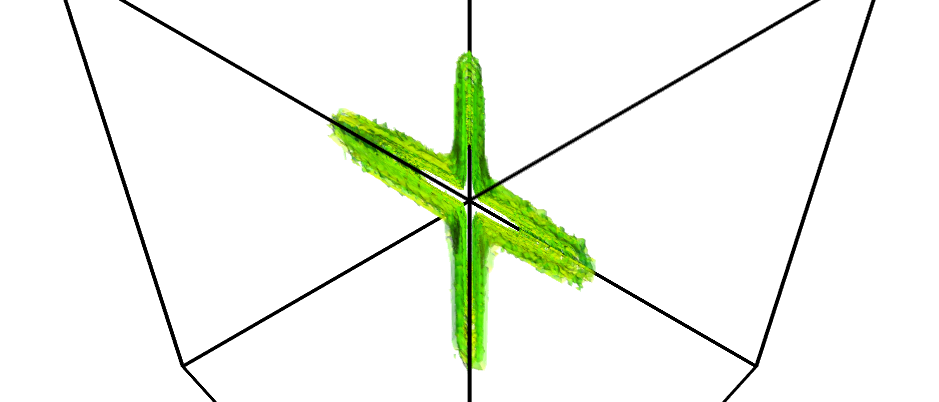
\includegraphics[width=1.in,trim={11.3cm 0cm 11.3cm 0cm},clip]{tube_dual_c6_x128_b64/x_19_scene1.png}} 
 \fbox{ 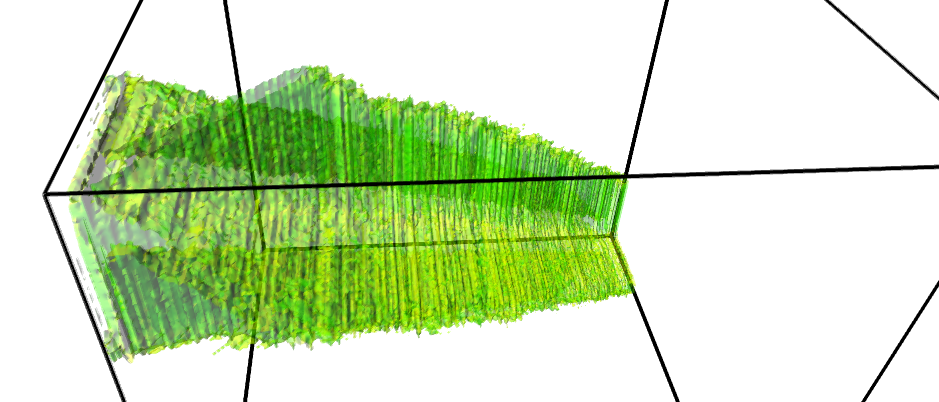
\includegraphics[width=2.in,trim={2cm 0cm 10cm 0cm},clip]{tube_dual_c6_x128_b64/x_19_scene2.png}} 
 \caption{Views of the $\tau =0.03$ sign occlusion surface, for the 
 128x~u.c.~nanotube, at $\sim {14k \times 14k}$ and $\kappa(\mat{s})=10^6$. 
 This surface envelopes the $ijk$ volume of the $\ot$ kernel,  
 cooresponding to the unscaled dual iteration step $\mmat{x}_{19} \leftarrow \mmat{y}_{19} \ot \mmat{z}_{19} $ at $b=64$, $\tau=0.03$ and
 $\tau_y=10^{-3} \, \tau $.  The first pannel looks straight down the cube-diagonal $i=j=k$, from the upper bound towards (1,1,1).
 Remarkably, this surface forms an elongated $\times$, closely following intersection of the $i=j$  and $i=k$ planes 
 along the cube-diagonal. The second pannel looks along the cube-diagonal, with the upper bound at upper left, and (1,1,1) at lower right.}
 \end{figure}

In this section, we present  numerical experiments that highlight the effects of 
ill-conditioning, dimensionality, and the stability of different first order NS approaches to iteration with $\tt SpAMM$. 
We turn first to complexity reduction for $\ot$ in the basin of stability,  where we find a novel, compressive 
effect in the product octree.  This effect is shown in Fig.~\ref{markofzorro},  
for unscaled, inverse square root duals iteration, Eqs.~(\ref{dualsiteration}), on the 3,3 carbon 
nanotube metric at $\kappa=10^6$.  

In this example, the $\tt SpAMM$ octree culled from the $ijk$-cube is outlined by its occlusion surface, enclosing 
a volume that closely follows the $i=j$ and $i=k$ planes, forming an $\times$.  The banded distribution
of large norms along  matrix diagonals leads to cube-diagonal dominance, with plane-following 
a consequence of moderate ill-conditioning,  large norms along the plane-diagonals and their overlap in $ijk$
via the multiplicative bound, Eq.~(\ref{bound}). The tightness of this bound, and the compression gained relative
to  methods that control only the absolute error, {\em e.g.} as given by Eq.~(\ref{sparseapprox}), will hopefully
be quantified in future work. 





\begin{figure}[h]
  \caption{equation...}
\fbox{ 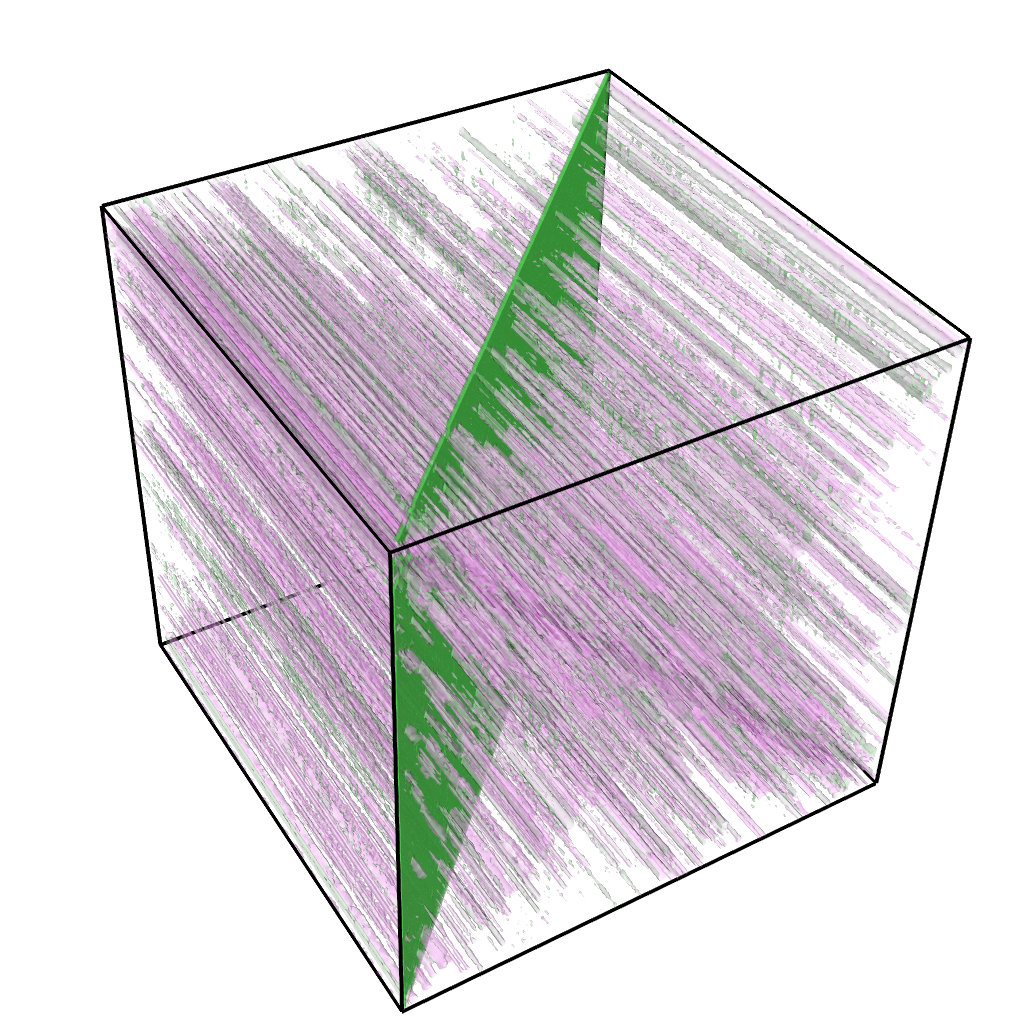
\includegraphics[width=1.5in,trim={6cm 6cm 6cm 6cm},clip]{y_15_water.png}} 
\fbox{ 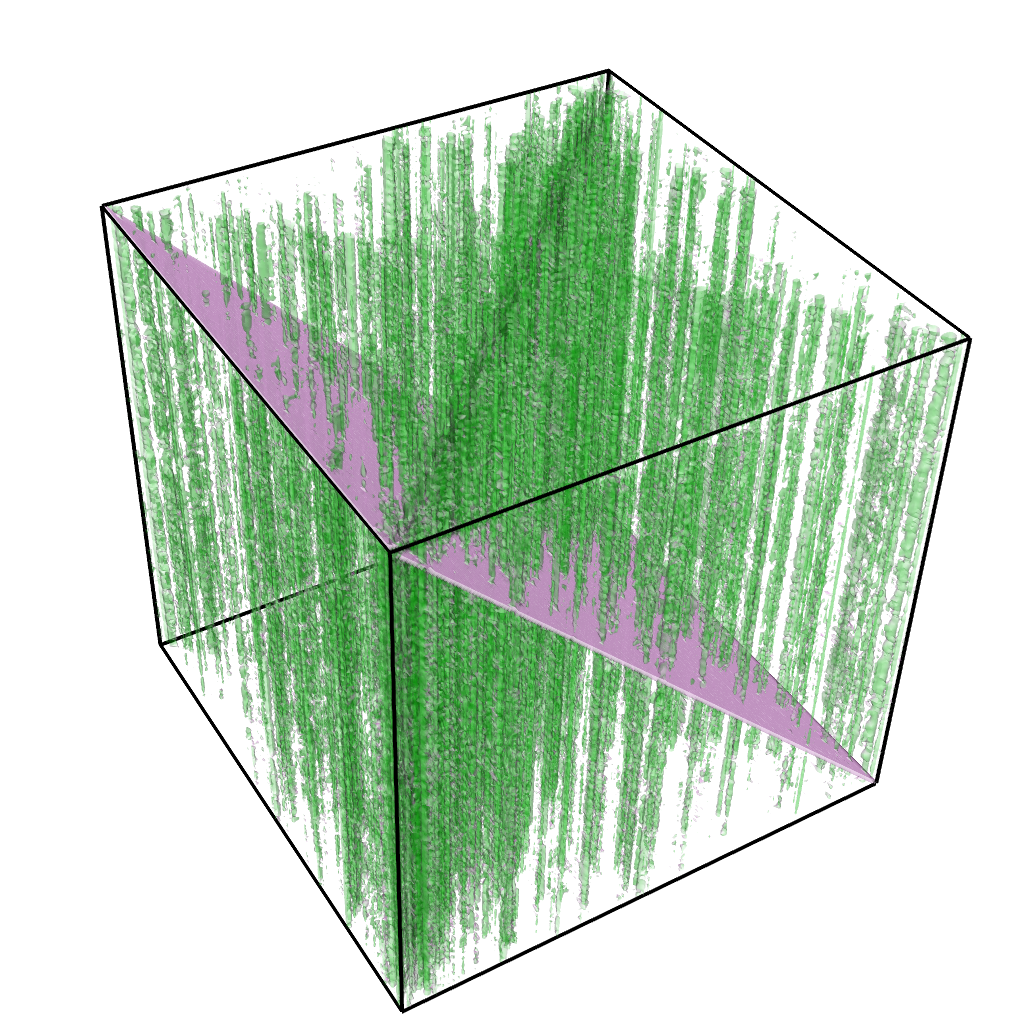
\includegraphics[width=1.5in,trim={6cm 6cm 6cm 6cm},clip]{z_15_water.png}}
\end{figure}



\begin{figure}[h]
  \caption{equation...}
%%\fbox{ \includegraphics[width=1.5in,trim={6cm 6cm 6cm 6cm},clip]{y_water_to_duals.png}} 
%%\fbox{ \includegraphics[width=1.5in,trim={6cm 6cm 6cm 6cm},clip]{z_water_to_duals.png}}
%\fbox{ \includegraphics[width=1.5in,trim={6cm 6cm 6cm 6cm},clip]{y_water_to_duals.png}} 
\fbox{ \includegraphics[width=3in,trim={8cm 0.1cm 8cm 0.1cm},clip]{z_water_to_duals_scn1.png}}
\end{figure}


\subsection{error flows}

\begin{figure}[h]
 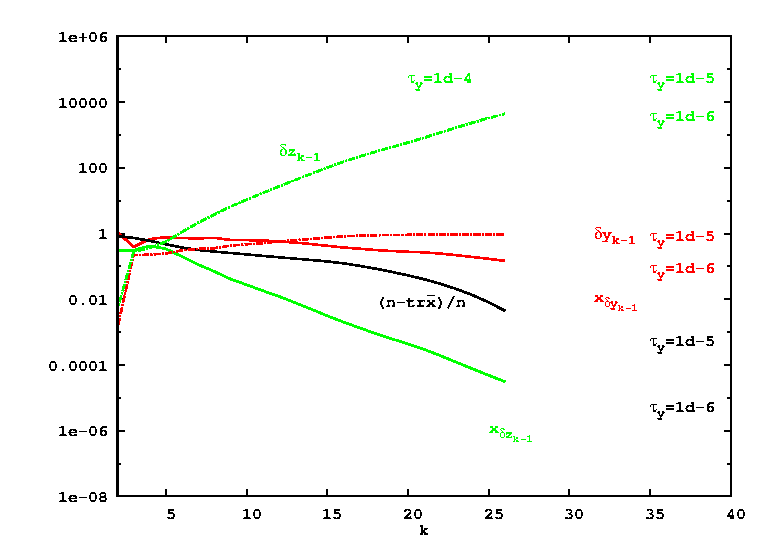
\includegraphics[width=3.5in]{33_nanotube_cond10_noscale_stab.eps}
\caption{Derivatives, displacements and the approximate trace of the unscaled, stablized NS iteration for a (3,3) nanotube with $\kappa =10^{10}$. 
Derivatives are full lines, whilst the displacements cooresponding to $\tau=10^{-3}$ and $\tau_y=\{10^{-4}, 10^{-5}, 10^{-6}\}$  
are the dashed lines.  The trace expectation is shown as a full black line. }
\end{figure}


\begin{figure}[h]
 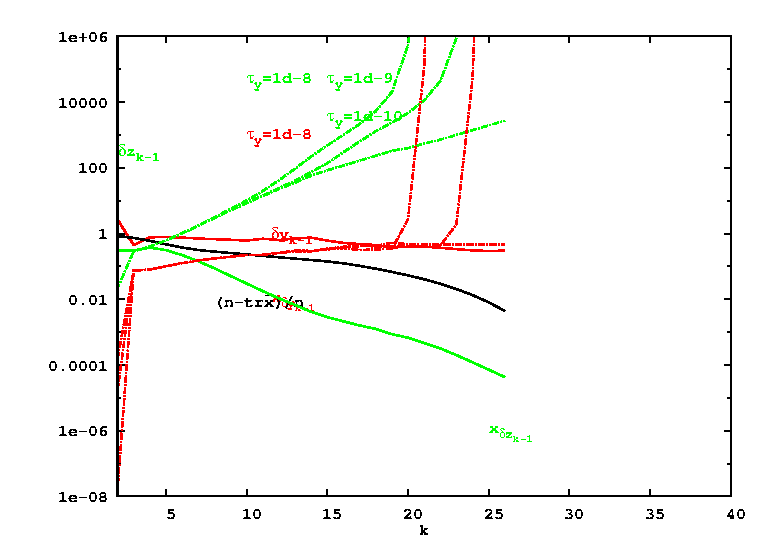
\includegraphics[width=3.5in]{33_nanotube_cond10_noscale_dual.eps}
\caption{Derivatives, displacements and the approximate trace of the unscaled, dual NS iteration for a (3,3) nanotube with $\kappa =10^{10}$. 
Derivatives are full lines, whilst the displacements cooresponding to $\tau=10^{-3}$ and $\tau_y=\{10^{-8}, 10^{-9}, 10^{-10}\}$  
are the dashed lines.  The trace expectation is shown as a full black line. }
\end{figure}



\section{Conclusion}

%%eg vs row-col picture.  Example of exact exchange w/DBSR 

\bibliography{MatrixFunctions}

\end{document}
